Bei der Entwicklung mit den Arduino Boards wurde die Arduino IDE eingesetzt.
Mit der Programmiersprache C und ein paar Bibliotheken ist es somit sehr schnell möglich, funktionierenden Code zu schreiben.
Bei der Entwicklung mit dem Pretzelboard wurde speziell die Bibliothek Softwareserial.h eingesetzt.
Diese ermöglicht es, direkt Befehle über die serielle Schnittstelle auszuführen.
Dabei gibt es einen Satz von vordefinierten Befehlen welche verwendet werden können.
Wenn z.bsp das Kommando 
\begin{lstlisting}
AT
\end{lstlisting}
an den seriellen Port gesendet wird, wird überprüft ob das Modul einsatzfähig ist.
Sollte dies der Fall sein, gibt das Kommando OK zurück.
Die Kommandos können jedoch auch deutlich komplexer Aufgaben mit einfach Kommandos abdecken.
So ist es auch möglich mit den folgenden Befehlen
\begin{lstlisting}
AT+CWMODE=1
AT+CWJAP="SSID","PASSWORD"
\end{lstlisting}
eine Verbindung mit einem WLAN Netzwerk aufzubauen.

Bei der Entwicklung mit Hilfe der Arduino IDE, werden 2 Prozeduren vordefiniert.
Einmal eine "`setup"' Prozedur, welche direkt nach dem starten des Buttons ausgeführt wird.
In der Prozedur sollte Code ausgeführt werden, welche nur Initial benötigt wird, wie etwa das verbinden mit einem WLAN Netzwerk.
Die zweite Standard Prozedur wird "`loop"' genannt.
Wie der Name schon sprechend sagt, wird der Code hier in einer Schleife ausgeführt.
Hier bietet es sich an, z.bsp. den Staus eines Button abzufragen.

Bei der Entwicklung des Codes wurde ein Großteil der Logik in Unterprozeduren geschrieben, welche dann in den genannten Hauptprozeduren ausgeführt werden.
So wird in der "`setup"' Prozedur mithilfe der Prozedur "`configAP"' eine Verbindung mit dem WLAN Netzwerk aufgebaut und anschließend wird mit der Prozedur "`configUDP"' eine Verbindung mit dem UDP Server des Raspberry Pis hergestellt.
In der "`loop"' Prozedur wird hingegen nur der Status des Buttons überprüft.
Wird festgestellt, das dieser gedrückt wurde, wird per UDP die ID des Buttons gesendet. 
(siehe Anhang \ref{sec:CodePretzelboard})

\begin{figure}[H]
	\centering
	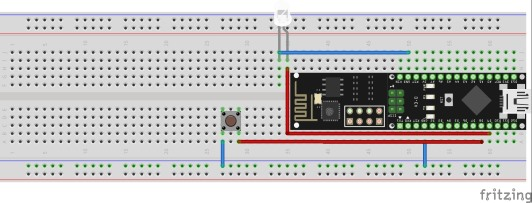
\includegraphics[scale=1.5]{Pretzel_Fritzing.jpg}
	\caption[Pretzelboard Versuchsaufbau]{Pretzelboard Versuchsaufbau,\\ Quelle: Eigener Entwurf mit Hilfe des Tools Fritzing (vgl. \cite{.fritz})}
\end{figure}